\documentclass{article}
\usepackage{amsmath}
\usepackage{graphicx}

\begin{document}

\section*{Figuring out what happens with the solver when there is
  attenuation}

I like to use simple test cases because they clarify to me what is
\textit{not} the problem. So I will be considering the following
situation: a $1\times 1\times 1$ meter box, and I will be evaluating
the solution at the center of that cube. The left face of the cube is
marked as a port, as is the right. So the equations we will be
solving when we are driving the left port are:
\begin{align*}
  -\omega^2 p(x,y,z) - c^2 \Delta p(x,y,z) &= 0, \\
  p(x=0,y,z) &= 1, && \text{(left boundary)}\\
  p(x=1,y,z) &= 0, && \text{(right boundary)} \\
    \frac{\partial p}{\partial n} &= 0,
     && \text{(all other boundaries)}
\end{align*}
The wave speed is computed as
\begin{align*}
  c = \sqrt{\frac{K}{\rho}},
\end{align*}
where $K$ is the bulk modulus and $\rho$ is the density, both of which
are read from the input file as frequency-dependent quantities, and
which can both be complex-valued.


\subsection*{Testing the pressure}

The set-up is chosen so that the solution is one-dimensional. As a
consequence, the solution only depends on $x$ and we can easily derive
it as
\begin{align*}
  p(x,y,z) = p(x) &= \frac{e^{jkx} - e^{-jk(2L-x)}}{1 - e^{-2jkL}},
\end{align*}
with $L=1$ and $k=\frac{\omega}{c}$. It is not difficult to verify
that indeed the boundary conditions are satisfied:
\begin{align*}
  p(0) &= \frac{e^{jk0} - e^{-jk(2L-0)}}{1 - e^{-2jkL}}
  =
  \frac{1 - e^{-2jkL}}{1 - e^{-2jkL}} = 1,
  \\
  p(L) &= \frac{e^{jkL} - e^{-jk(2L-L)}}{1 - e^{-2jkL}}
  = \frac{e^{jkL} - e^{-jkL}}{1 - e^{-2jkL}} = 0.
\end{align*}
It is also not difficult to check that the equation itself is
satisfied:
\begin{align*}
  -\omega^2 p(x) - c^2 \Delta p(x)
  &= -\omega^2 p(x) - c^2 p''(x)\\
  &= -\omega^2 p(x) - c^2 (jk)^2 p''(x)  \\
  &= (k^2c^2-\omega^2) p(x) \\
  &= \left(\frac{\omega^2}{c^2}c^2-\omega^2\right) p(x)\\
  &= 0.
\end{align*}

With this solution, evaluated at the center of the box of length
$L=1$, we obtain
\begin{align*}
  p_\text{center} &= p(0.5)
  \\
  &= \frac{e^{\frac{jk}{2}} - e^{-\frac{3jk}{2}}}{1 - e^{-2jk}}
  \\
  &= \frac{e^{\frac{jk}{2}} - e^{-\frac{3jk}{2}}}{e^{jk} - e^{-jk}}
  \\
  &= \frac{e^{\frac{j\omega}{2c}} - e^{-\frac{3j\omega}{2c}}}{1 - e^{-\frac{2j\omega}{c}}}
  \\
  &= \frac{e^{\frac{j\omega}{2}\sqrt{\frac{\rho}{K}}} - e^{-\frac{3j\omega}{2}\sqrt{\frac{\rho}{K}}}}{1 - e^{-2j\omega\sqrt{\frac{\rho}{K}}}}
\end{align*}
We will consider this expression for two special cases below, without
and with attenuation.


\subsubsection*{No attenuation}

Let us consider the evaluation of the pressure at the center of the
box for the special case without attenuation. For simplicity, we
choose $\rho=K=1$ and consequently $c=1$ and $k=\omega$. Then, based
on the formulas in the \texttt{readme.md} file at the top level of the
github repository, we have
\begin{align*}
  p(x)
  &=
  \frac{e^{jkx} - e^{-jk(2L-x)}}{1 - e^{-2jkL}}.
\end{align*}
This formula, after a good bit of massaging, can be restated as
follows for real-valued $k$:
\begin{align*}
  p(x)
  &=
  \frac{\sin(k(L-x))}{\sin(kL)}.
  \\
  &=
  \frac{\sin(\omega(1-x))}{\sin(\omega)}.
\end{align*}
This expression, unsurprisingly, has singularities for
$\omega=\pi,2\pi,3\pi,...$, where the cavity is in resonance. This
corresponds to frequencies $f=0.5, 1, 1.5, \ldots$ Hertz. As a
consequence, we better consider frequences below the first resonance,
i.e., $\omega<\pi$, i.e., $f<0.5$ Hertz.

That said, for the specific case of the center of the box (at $x=0.5$), we get
\begin{align*}
  p_\text{center}
  &= 
  \frac{\sin(\omega/2)}{\sin(\omega)}.
\end{align*}
In the low-frequency case, $\omega\ll 1$, we have the asymptotic
behavior
\begin{align*}
  p_\text{center}
  &\approx
  \frac{\omega/2}{\omega}
  = \frac 12.
\end{align*}

We can plot what the program produces for a number of frequencies in
the range between 0.1 and 1 Hz:
%
% dii_frequency_response.csv, columns 1 (frequency), 14 (real part of
% pressure), 15 (imaginary part of pressure)
%

{\centering
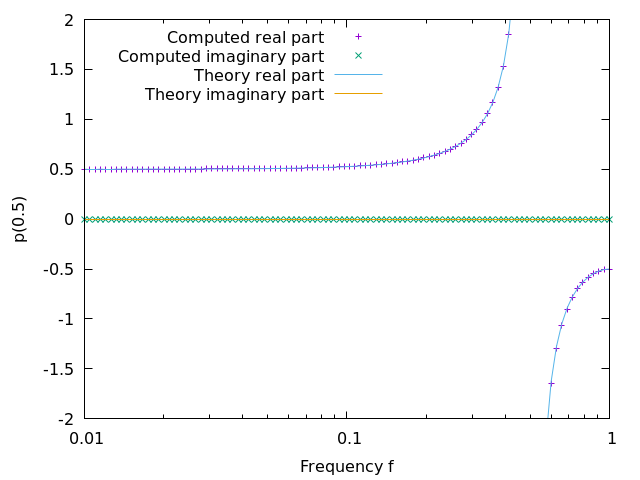
\includegraphics[width=0.7\textwidth]{no-attenuation/pressure-at-center.png}
}

As can be seen, the computations (shown as the blue crosses) are an
excellent match for the expected theoretical behavior. Furthermore,
the singularity (resonance) is at $f=0.5$ Hz, again as expected.

\end{document}
